\documentclass{article}
\usepackage{float}
\usepackage{graphicx} % Required for inserting images with \includegraphics command.
\usepackage[hidelinks]{hyperref} % Required in order to use in-page links in the table of contents
                                 % Option "hidelinks" used to hide links border in some pdf reader such as Acrobat Reader.

%Package imported in order to customize cells in tabularx environment. In particular was
%added to allow the use of "\\" syntax inside a table's cell.
\usepackage{makecell}

%Packages and instruction to change scale of sections', subsections' and subsubsections' heads
\usepackage{titlesec}
\usepackage{titlesec}
%Makes sections' contents in bold, and increases their sizes.
\titleformat*{\section}{\Huge\bfseries}
%Same thing as above but for subsections
\titleformat*{\subsection}{\LARGE\bfseries}
%Same thing as above but for subsubsections
\titleformat*{\subsubsection}{\Large\bfseries}

%Instruction used to create a new subsection level (subsubsubsection) in the document
\titleclass{\subsubsubsection}{straight}[\subsection]
%Instructions used to create a new counter (used to count the number of subsubsubsections
%within a subsubsection) for the subsubsubsections and creation of the command to invoke(use) them
\newcounter{subsubsubsection}[subsubsection]
\renewcommand\thesubsubsubsection{\thesubsubsection.\arabic{subsubsubsection}}

%Instruction used to align the new section layer in a correct manner in the table of contents
%Without this subsubsubsections would remain on the same line, creating a mess in the table of
%contents.
\makeatletter

%Instructions to change the scale and font of the subsubsubsections' head
\titleformat{\subsubsubsection}
  {\normalfont\large\bfseries}{\thesubsubsubsection}{1em}{}
\titlespacing*{\subsubsubsection}
{0pt}{3.25ex plus 1ex minus .2ex}{1.5ex plus .2ex}

%Instructions to create the subsubsubsections entries in the table of contents (included the dot line)
\def\toclevel@subsubsubsection{4}
\def\l@subsubsubsection{\@dottedtocline{4}{7em}{4em}}

%Instruction used to restore "@" symbol to "other" instead of a "latter" made by
%\makeatletter command. Just a safety command useful for latex but not of our interest.
\makeatother

%Instructions to set table of contents and sections depth to 4 layers (in order to include even
%subsubsubsections).
\setcounter{secnumdepth}{4}
\setcounter{tocdepth}{4}

%Used in order to have more symbols for itemize lists (in our case the "arrow" symbol in phenomena section)
\usepackage{pifont}

%Used to make the header and footer of each document page
\usepackage{fancyhdr}

%Defines a new style of header and footer
%Defines the content of the header and the footer of the pages of the first section
\fancypagestyle{IntroductionStyle}{
\fancyhf{}
\fancyhead[L]{\textit{\textbf{SECTION 1. INTRODUCTION}}}
\fancyfoot[L]{CKB \quad - \quad \textbf{D}esign \textbf{D}ocument}
\rfoot{\thepage}
\renewcommand{\headrulewidth}{0.4pt}
\renewcommand{\footrulewidth}{0.4pt}
}
%Defines the content of the header and the footer of the pages of the second section
\fancypagestyle{OverallDescriptionStyle}{
\fancyhf{}
\fancyhead[L]{\textit{\textbf{SECTION 2. ARCHITECTURAL DESIGN}}}
\fancyfoot[L]{CKB \quad - \quad \textbf{D}esign \textbf{D}ocument}
\rfoot{\thepage}
\renewcommand{\headrulewidth}{0.4pt}
\renewcommand{\footrulewidth}{0.4pt}
}
%Defines the content of the header and the footer of the pages of the third section
\fancypagestyle{SpecificRequirementsStyle}{
\fancyhf{}
\fancyhead[L]{\textit{\textbf{SECTION 3. USER INTERFACE DESING}}}
\fancyfoot[L]{CKB \quad - \quad \textbf{D}esign \textbf{D}ocument}
\rfoot{\thepage}
\renewcommand{\headrulewidth}{0.4pt}
\renewcommand{\footrulewidth}{0.4pt}
}
%Defines the content of the header and the footer of the pages of the fourth section
\fancypagestyle{FormalAnalysisAlloyStyle}{
\fancyhf{}
\fancyhead[L]{\textit{\textbf{SECTION 4. REQUIREMENTS TRACEABILITY}}}
\fancyfoot[L]{CKB \quad - \quad \textbf{D}esign \textbf{D}ocument}
\rfoot{\thepage}
\renewcommand{\headrulewidth}{0.4pt}
\renewcommand{\footrulewidth}{0.4pt}
}
%Defines the content of the header and the footer of the pages of the fifth section
\fancypagestyle{EffortSpentStyle}{
\fancyhf{}
\fancyhead[L]{\textit{\textbf{SECTION 5. IMPLEMENTATION, INTEGRATION, TEST PLAN}}}
\fancyfoot[L]{CKB \quad - \quad \textbf{D}esign \textbf{D}ocument}
\rfoot{\thepage}
\renewcommand{\headrulewidth}{0.4pt}
\renewcommand{\footrulewidth}{0.4pt}
}
%Defines the content of the header and the footer of the pages of the sixth section
\fancypagestyle{ReferencesStyle}{
\fancyhf{}
\fancyhead[L]{\textit{\textbf{SECTION 6. EFFORT SPENT}}}
\fancyfoot[L]{CKB \quad - \quad \textbf{D}esign \textbf{D}ocument}
\rfoot{\thepage}
\renewcommand{\headrulewidth}{0.4pt}
\renewcommand{\footrulewidth}{0.4pt}
}
%Defines the content of the header and the footer of the pages of the seventh section
\fancypagestyle{ReferencesStyle}{
\fancyhf{}
\fancyhead[L]{\textit{\textbf{SECTION 7. REFERENCES}}}
\fancyfoot[L]{CKB \quad - \quad \textbf{D}esign \textbf{D}ocument}
\rfoot{\thepage}
\renewcommand{\headrulewidth}{0.4pt}
\renewcommand{\footrulewidth}{0.4pt}
}

%Used to handle table width and split tables across different pages
\usepackage{xltabular}
%Change space between table columns
\setlength{\tabcolsep}{18pt}

%Command used to create a new column type whose background is lightgray colored
\usepackage{xcolor,colortbl}
\definecolor{LightGray}{gray}{0.85}
\newcolumntype{g}{>{\columncolor{LightGray}}c}


%Set the default path of images (used in includegraphics command)
\graphicspath{ {images/} }

\title{\Huge{\textbf{Design Document}}}
\author{\Large{Francesco Spangaro - Tosetti Luca - Francesco Riccardi}}
\date{07 January 2024}

\begin{document}

\maketitle

\begin{figure}[h]
    \centering
    
\includegraphics[scale=0.6]{politecnico-di-milano-logo.png}
\end{figure}

\vspace*{1cm}
\begin{center}
      \Large{\textbf{Prof.}} \\
      \Large{\textbf{Matteo Camilli}}
\end{center}
\vspace*{1cm}

\begin{center}
      \large{Version 0.1} \\
      \large{Academic Year 2023 - 2024}
\end{center}

\tableofcontents

\newpage
\pagestyle{IntroductionStyle}

\section{Introduction}
\subsection{Purpose}
The purpose of this document is to provide an exhausting and implementative
description of the platform that will be implemented (CKB platform).
In particular the document is focused on the description of the architectural styles and decisions
that will be adopted, the modules that compose the platform and their interfaces.
The document will contains also several details regarding the deployment choices,
the runtime view of the core functionalites of the platform that will be used in it.
The document contains some mockups of the user interface design.
The document also covers the implementation, integration and testing
processes required to implement correctly the CKB platform.
\subsection{Scope}
CodeKataBattle (CKB) is a platform which aims to give to Educators an easy-to-use experience, and let
them propose homework and/or lessons in a new and fresh way.
The main goal of the platform is to give the Students the possibility to improve and acquire new software
developing skills by particpating to several battles in as many tournaments.
The platform let Educators of the Students to create such tournaments and battles within them
in order to challenge the Students to upload the best possible solution to the battle's
problem. That solution will be then automatically evaluated by the platform which will give it a score,
and eventually even by the Educator who created the battle, and will be associated to it a proper score.
The platform also allow Educators to add several recognition badges for the work done by the students.
This badges can be personalized by the Educators themselves.
\\ \\
From the architectural point of view we have decided to adopt a 4-Tier Client-Server architecture combined
with a MSA server side, in addition to a MVC software architectural choice.
\subsection{Definitions, acronyms, abbreviations}
\subsubsection{Definitions}
{\renewcommand{\arraystretch}{1.5}
%\textwidth used to set table's width according to text's width of the page
%">{\raggedright\arraybackslash} c" used to align to the right the column c
%"X" column tag creates a paragraph-like column whose width automatically expands so that the declared width of the environment is filled
\begin{xltabular}{\textwidth}{ >{\raggedright\arraybackslash}c >{\raggedright\arraybackslash}X }
    \hline
    \textbf{Term} & \textbf{Definition} \\
    \hline

    \endfirsthead   %Everything above is used as "head" (first row) of
    %the table in the page where it is placed

    \hline
    \textbf{Term} & \textbf{Definition} \\
    \hline

    \endhead    %Everything above is used as "head" (first row) of the
    %splitted parts of the table in the pages different from
    %the one in which the table was originally placed

    \endfoot    %Everything above is used as "foot" (last row) of the
    %splitted parts of the table in the pages different from
    %the last one in which the table appear

    \endlastfoot    %Everything above is used as "foot" (last row) of the
    %table in the page where it appears last.

    \textit{4-Tier Architecture} & $\rightarrow$ A 4-Tier architecture in the field of informatic systems, very simply
    a software and hardware architecture in which a running application/platform is divided in four different modules
    or also called "layers" which usually are: Presentation Layer, WebServer layer, Logic Layer, Data Layer. \\
    \textit{Presentation Layer} & $\rightarrow$ The top layer of the 4-Tier architecture. It takes care of the interaction
    between the user and the application.\\
    \textit{WebServer Layer} & $\rightarrow$ The second layer of the 4-Tier architecture. It takes care of handling the requests
    sent by the users throught a browser application. \\
    \textit{Logic Layer} & $\rightarrow$ The third layer of the 4-Tier architecture. It takes care of implementing the real
    application logic that allows to the application/platform to actually work. \\
    \textit{Data Layer} & $\rightarrow$ The bottom layer of the 4-Tier architecture. It takes care of all the data generated
    by the users or the application, and with which the application itself has to interact. The interactions
    can include queries, updates, deletions, ... \\
    \textit{Microservice architecture} & $\rightarrow$ An architectural style that consist in the creation of an
    application/platform as a suite of small services, each one handling a part of the business logic of the application
    and that comunicates with each other throught lightweight protocols (such as HTTP). \\
    \textit{Model-View-Controller} & $\rightarrow$ An architectural pattern used to develop the
    software logic of an application. This pattern consist in dividing the application in three
    different parts: View, Model and Controller. \\
    \textit{View} & $\rightarrow$ Part of the MVC pattern which takes care of the visualization of the
    data contained in the model and the interaction with the user. \\
    \textit{Controller} & $\rightarrow$ Part of the MVC pattern that receives commands from the user, and execute them
    by modifying the View and/or Model parts. \\
    \textit{Model} & $\rightarrow$ Part of the MVC pattern that gives to the Controller part, the
    methods to access the application's data and to modify them.
\end{xltabular}

\subsubsection{Acronyms}
\begin{xltabular}{\textwidth}{ >{\raggedright\arraybackslash}c >{\raggedright\arraybackslash}X }
    \hline
    \textbf{Acronym} & \textbf{Meaning} \\
    \hline

    \endfirsthead

    \hline
    \textbf{Acronym} & \textbf{Meaning} \\
    \hline

    \endhead
    \endfoot
    \endlastfoot

    \textit{MSA} & $\rightarrow$ MicroServices Architecture\\
    \textit{MVC} & $\rightarrow$ Model-View-Controller\\
    \textit{RASD} & $\rightarrow$ Requirement Analysis and Specification Document\\
    \textit{DD} & $\rightarrow$ Design Document\\
    \textit{CKB} & $\rightarrow$ CodeKataBattle\\
    \textit{} & $\rightarrow$ \\
\end{xltabular}


\subsubsection{Abbreviations}
\begin{xltabular}{\textwidth}{ >{\raggedright\arraybackslash}c >{\raggedright\arraybackslash}X }
    \hline
    \textbf{Abbreviation} & \textbf{Meaning} \\
    \hline

    \endfirsthead

    \hline
    \textbf{Abbreviation} & \textbf{Meaning} \\
    \hline

    \endhead
    \endfoot
    \endlastfoot

    \textit{e.g.} & $\rightarrow$ Exempli gratia, latin phrase meaning "for example".
    \\
    \textit{} & $\rightarrow$
    \\
    \textit{} & $\rightarrow$
    \\
    \textit{} & $\rightarrow$
    \\
    \textit{} & $\rightarrow$
    \\
\end{xltabular}
\subsection{Revision history}
\begin{itemize}
    \item **Placeholder data**: version 1.0
\end{itemize}

\subsection{Reference documents}
UML official specification $\rightarrow$ \url{https://www.omg.org/spec/UML}
\\ \\
Sequence diagrams specification $\rightarrow$ \url{https://www.uml-diagrams.org/sequence-diagrams.html}
\\ \\
Component diagrams specification $\rightarrow$ \url{https://creately.com/blog/software-teams/component-diagram-tutorial/}
\\ \\
Deployment diagrams specification $\rightarrow$ \url{https://pubs.opengroup.org/architecture/archimate32-doc.singlepage/}
\subsection{Document structure}
\begin{itemize}
    \item \textbf{\textit{Section 1: Introduction}} \\
          This section offers a brief description of the problem and the platform/application that will be developed in order to resolve it.
          It describes the major purpose of this document, a very brief recap of the domain which is
          described in detail in the RASD document.
          In addition, in this section are inserted definitions, acronyms and abbreviations used in the document,
          its revision history and refereced documents or web pages.
    \item \textbf{\textit{Section 2: Architectural Design}} \\
          This section is the main part of the document. It describes the architectures used to
          realize the platform, the CKB platform's components, its interfaces, its deployment
          structure and finally its runtime behaviour.
          All these aspects are described through several diagrams such as:
          component diagrams, class diagrams, deployment diagrams and other
          generic diagrams which are used to give a representation of main and most important
          features of the platform.
    \item \textbf{\textit{Section 3: User interface design}} \\
          This section describes the user interface design of the platform.
          It contains several mockups of the interface that the Educators and
          Students will find when they access to the platform. The presented mockups
          refers to the client-side experience throught an appropriate browser application.
    \item \textbf{\textit{Section 4: Requirements traceability}} \\
          This section describe the connection between the RASD and DD document,
          by providing a complete map of the requirements and goals expressed in the RASD
          to the modules presented in this document.
    \item \textbf{\textit{Section 5: Implementation, Integration \& Test plan}} \\
          This section describes the plan followed for implementing, testing and
          integrating the platform's components, the order in which
          these operations are performed and what they generate.
    \item \textbf{\textit{Section 6: Effort spent}} \\
          This section contains all the information about the time spent by each group member
          in order to complete this document and its division by each section of the document.
\end{itemize}
\section{Architectural Design}
\subsection{Overview: High-level components and interactions}
To ensure high maintainability, security and reliability, the service is structured by following the four-tier architecture model.
Figure 1. shows how the tiers are divided, and what are the relations between each tier of the system.
\begin{figure}[H]
    \centering
    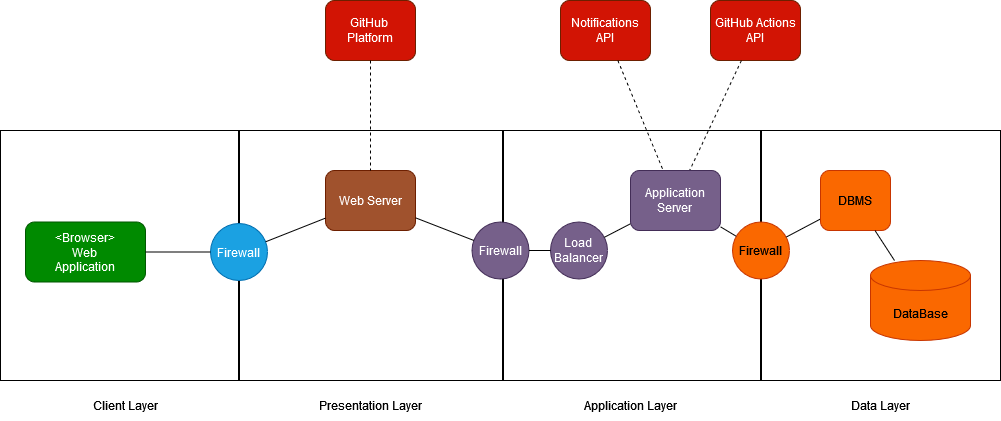
\includegraphics[scale=0.35]{images/FourTierApplication.png}
    \caption{Four-tier architecture}
    \label{fig:Figure 1}
\end{figure}
\noindent
The main components are: \\ \\
\textbf{Web Application:} The web application allows users to connect to the platform's services. The web application can be accessed by any device
that is connected to the internet and can browse the web. Students and Educators will have different views of the web application, because they have
different parameters that they can view and manage. \\ \\
\textbf{Web Server:} The web server is what manages the web application. It is connected directly to the GitHub Platform to give Educators the possibility
of seeing their Students' uploaded solutions. It is connected to the GitHub platform to also give Students the possibility of seeing their
solutions uploaded to the platform in real time. It is the main container for the JavaScript and general backend code for the platform.
The web server is connected to the Application server because it needs to be automatically updated when new grades for Students' solutions are generated
by the platform. \\ \\
\textbf{Application Server:} The application server is the main backend of the CKB Platform. It contains all the code needed for th eplatform to run
smoothly and without interruptions. It contains the logic needed to answer the API requests made by the users to the platform. It
automatically evaluates Students' solutions proposed via the GitHub platform and uploads the new grade to the web server. \\ \\
\textbf{DBMS:} The DBMS is the main interpreter between the CKB platform and the data stored onto the database. \\ \\
\textbf{DataBase:} The database stores all the information needed by the application. \\ \\
\textbf{External Services:} These services provide informations and funtionalities that the CKB platform alone could not provide.
These funtionalities include a \textit{GitHub actions API} that notifies the platform of the upload of a new Student's solution, a \textit{notification API}
that notify Students when a new tournament or a new battle in a tournament they are subscribed to is created and a connection to the \textit{GitHub platform}
since the code needs to be uploaded from the GitHub platform to the CKB platform automatically. \\
\subsection{Component view}
\begin{figure}[H]
    \centering
    \hspace*{-4.1cm}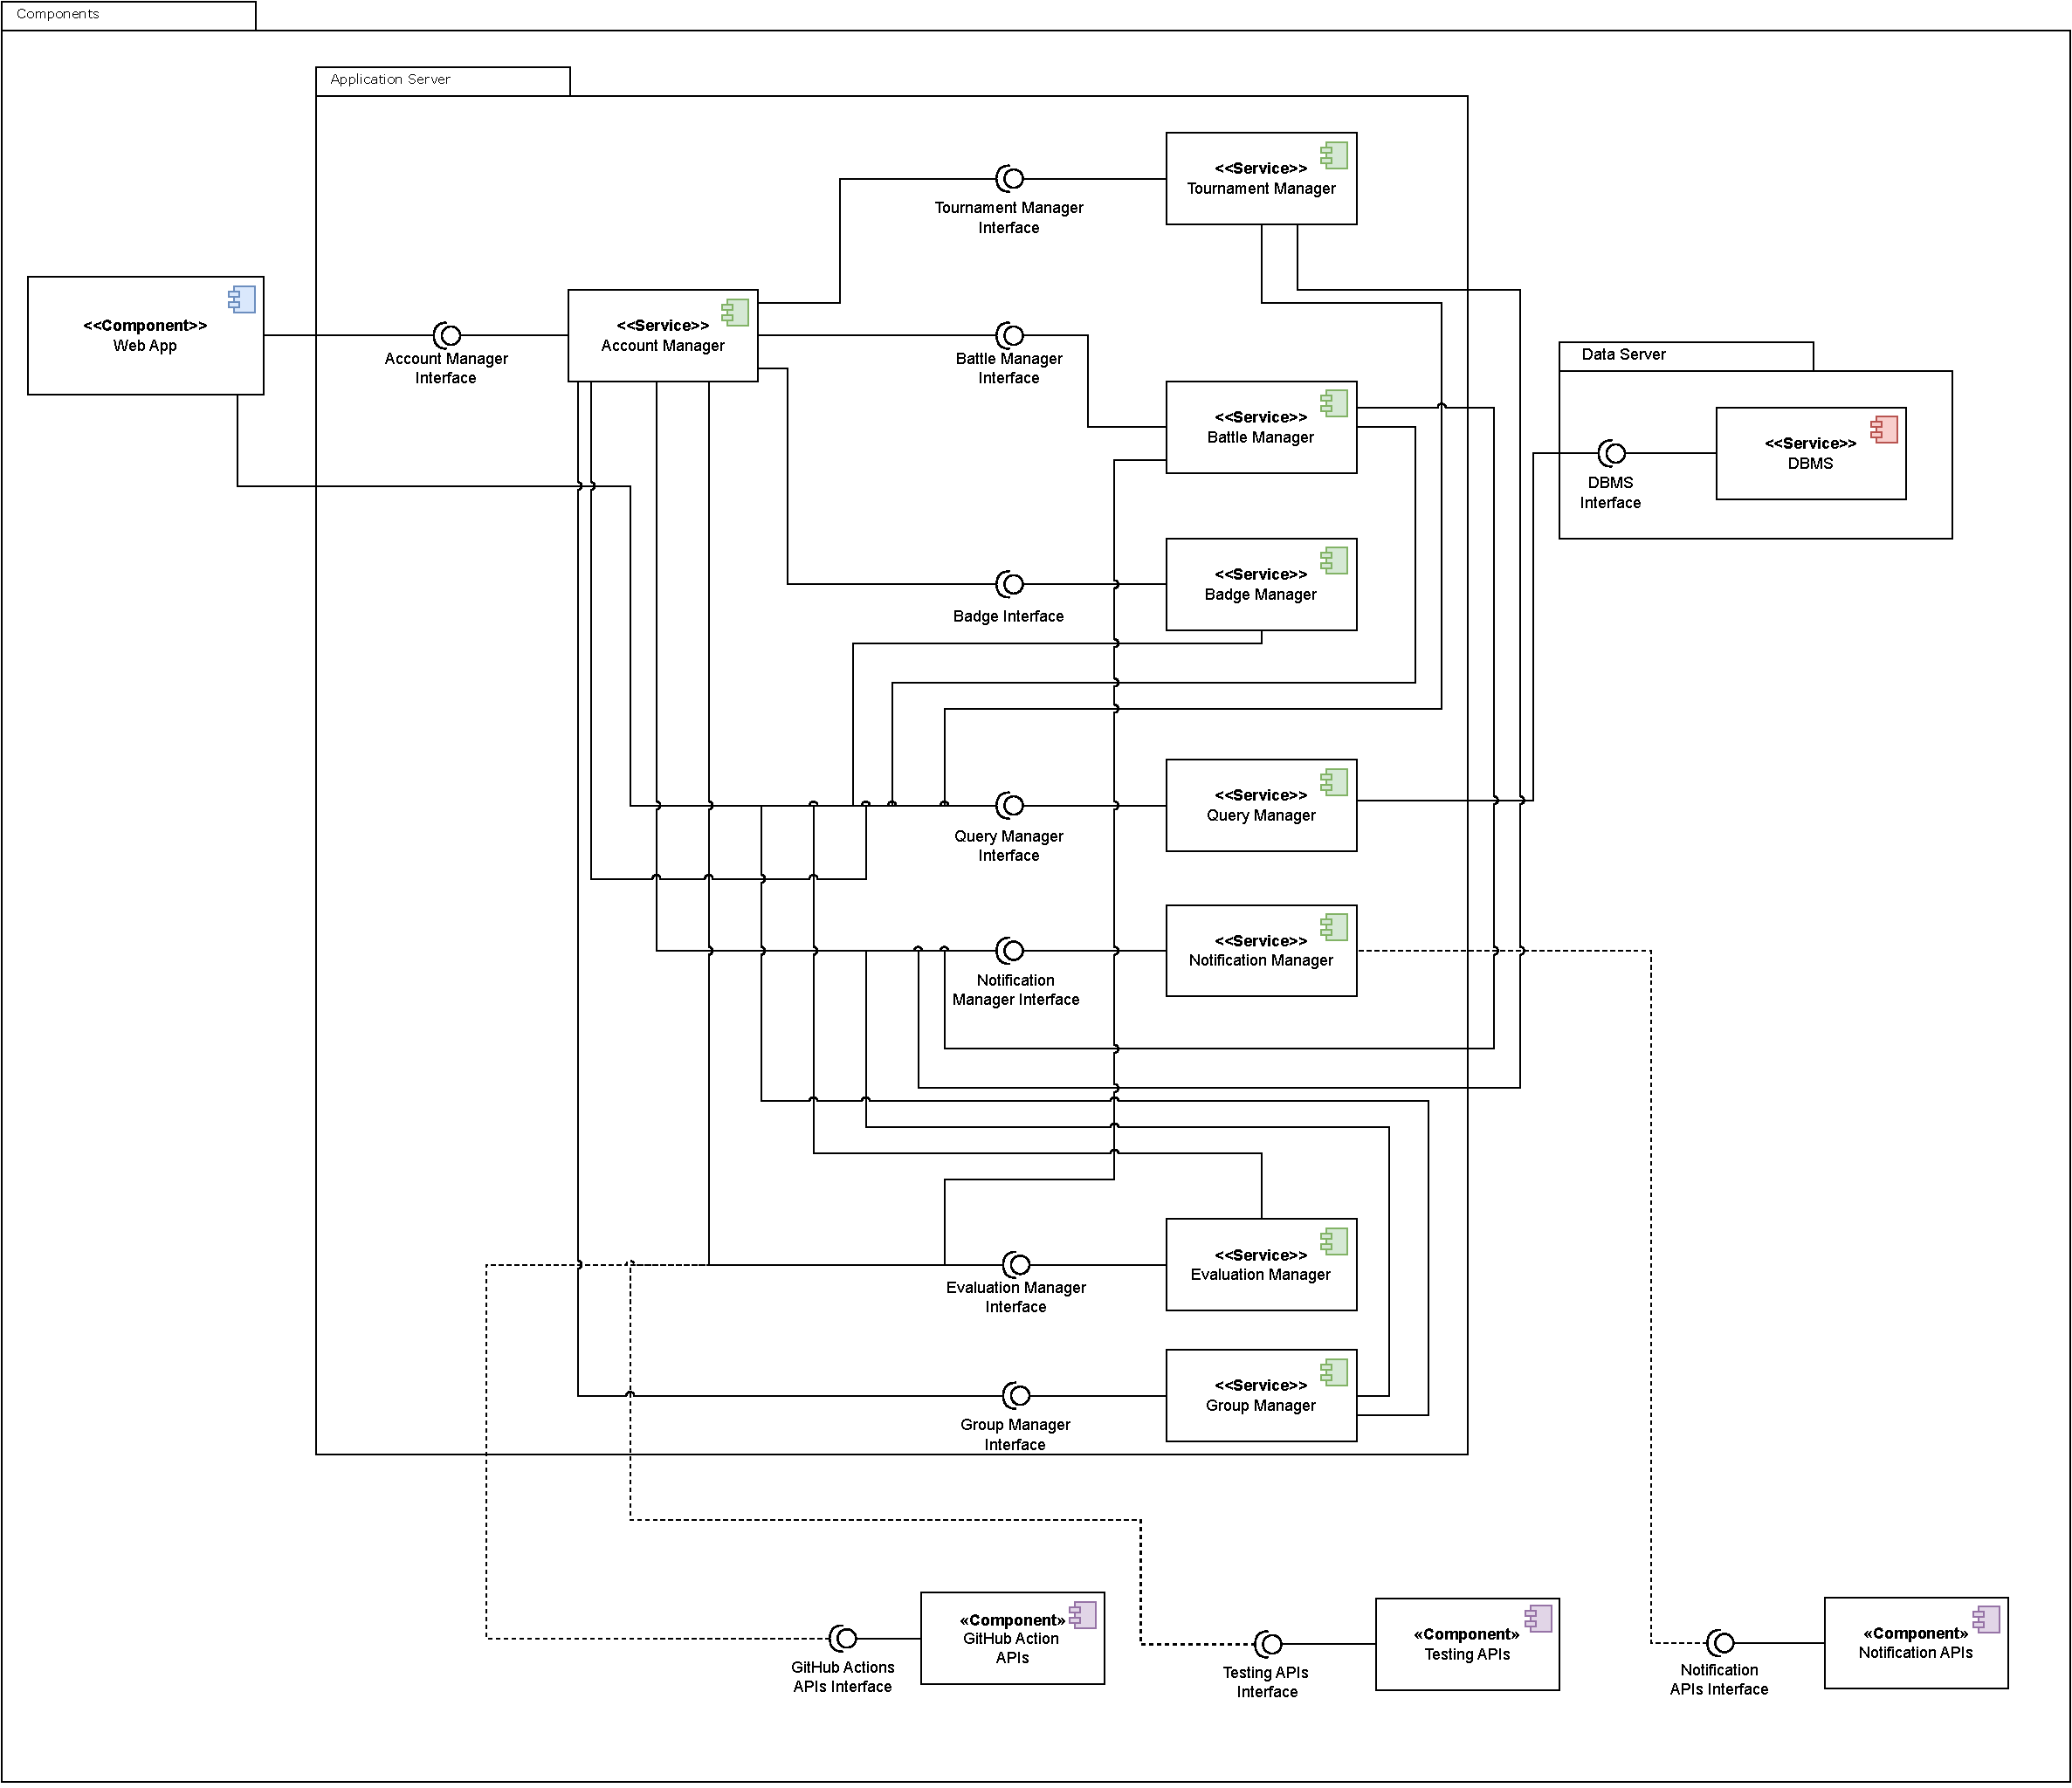
\includegraphics[scale=0.5]{images/ComponentView.pdf}
    \caption{Component diagram}
    \label{fig:classDiagram}
\end{figure}
In Figure 2 we can see a more detailed diagram, representing all the components previously described.
The Web App is what Students and Educator connect to via their web browsers.
It collects all of the Students' and Educators' requests, forwards them to the right service or component and sends back different responses.
\\
\textbf{Account Manager:}\\
\textbf{Tournament Manager:}\\
\textbf{Battle Manager:}\\
\textbf{Badges Manager:}\\
\textbf{Query Manager:}\\
\textbf{Notification Manager:}\\
\textbf{Evaluation Manager:}\\
\textbf{DBMS:}\\
\textbf{GitHub Actions APIs:}\\
\textbf{Testing APIs:}\\
\textbf{Notification APIs:}\\



\subsection{Deployment view}
\subsection{Component interfaces}
\subsection{Runtime view}
\subsection{Selected architectural styles and patterns}
\subsection{Other design decisions}
\section{User Interface Design}
\section{Requirements traceability}
\begin{itemize}
    \item \textbf{R.1:} The CKB platform should allow an
        unregistered Student to create a new account.
        \begin{itemize}
            \item \textbf{Account Manager:} Used to register or login to the platform.
            \item \textbf{Query Manager:} Used to store Students' informations after registration.
        \end{itemize}
    \item \textbf{R.2:} The CKB platform should allow an
        unregistered Educator to create a new account.
        \begin{itemize}
            \item \textbf{Account Manager:} Used to register or login to the platform.
            \item \textbf{Query Manager:} Used to store Educators' informations after registration.
        \end{itemize}
    \item \textbf{R.3:} The CKB platform must allow access to its pages only if the used credentials are correct.
        \begin{itemize}
            \item \textbf{Account Manager:} Used to check whether the credentials used are correct.
            \item \textbf{Query Manager:} Used to retrieve users' data.
        \end{itemize}
    \item \textbf{R.4:} The CKB platform must not allow a Student to register more than once in the system.
          \begin{itemize}
              \item \textbf{Account Manager:} Used to check if the Student has 
              already registered to the platform.
              \item \textbf{Query Manager:} Used to retrieve Student's data.
          \end{itemize}
    \item \textbf{R.5:} The CKB platform must not allow an Educator to register more than once in the system.
          \begin{itemize}
              \item \textbf{Account Manager:} Used to check if the Educator has already
              registered to the platform.
              \item \textbf{Query Manager:} Used to retrieve Educator's data.
          \end{itemize}
    \item \textbf{R.6:} Educators can access the platform's services only if they are registered to it.
          \begin{itemize}
              \item \textbf{Account Manager:} Used to check if the Educator is registered to
              the platform.
              \item \textbf{Query Manager:} Used to retrieve Educator's data.
          \end{itemize}
    \item \textbf{R.7:} Students can access the platform's services only if they are registered to it.
          \begin{itemize}
            \item \textbf{Account Manager:} Used to check if the Student is registered to
            the platform.
            \item \textbf{Query Manager:} Used to retrieve Student's data.
          \end{itemize}
    \item \textbf{R.8:} The CKB platform should not allow Students to create tournaments and/or battles.
          \begin{itemize}
              \item \textbf{Account Manager:} Used to check if the user is a Student and prevent him
              to access Tournament Manager APIs that should not have access to.
              \item \textbf{Query Manager:} Used to retrieve Student's data.
          \end{itemize}
    \item \textbf{R.9:} The CKB platform should allow Educators to create battles within a tournament only to the tournament
          creator and to any other Educator that has been granted permission to do so by the tournament creator.
          \begin{itemize}
              \item \textbf{Account Manager:} Used to check whether the logged Educator can create
              a battle within a certain tournament.
              \item \textbf{Battle Manager:} Used to create the new battle within the tournament.
              \item \textbf{Query Manager:} Used to retrieve Educator's data and eventually store battle's data
              just created.
          \end{itemize}
    \item \textbf{R.10:} The CKB platform must allow Educators to personalise the tournaments they create.
          \begin{itemize}
              \item \textbf{Tournament Manager:} Used to create and personalize new tournaments.
              \item \textbf{Query Manager:} Used to store tournament's data.
          \end{itemize}
    \item \textbf{R.11:} The CKB platform must allow Educators to personalise the battles they create.
          \begin{itemize}
              \item \textbf{Battle Manager:} Used to create and personalize new battles.
              \item \textbf{Query Manager:} Used to store battle's data.
          \end{itemize}
    \item \textbf{R.12:} The CKB platform must allow Educators to define new obtainable badges for each tournament they
          create.
          \begin{itemize}
              \item \textbf{Badges Manager:} Used to create new badges for a new tournament.
              \item \textbf{Query Manager:} Used to store badges data.
          \end{itemize}
    \item \textbf{R.13:} The CKB platform must allow Educators to manually evaluate the solutions uploaded by the Students for the battles that
          the Educators created.
          \begin{itemize}
              \item \textbf{Battle Manager:} Used to check whether the battle is enabled to be manually
              evaluated.
              \item \textbf{Evaluation Manager:} Used to allow the Educator to manually evaluate Students'
              work.
              \item \textbf{Query Manager:} Used to retrieve Educator and battle's data. Used to store
              scores given by the Educator through the manual evaluation.
          \end{itemize}
    \item \textbf{R.14:} The CKB platform must allow Educators to delete or update badges before finalizing a tournament's creation.
          \begin{itemize}
              \item \textbf{Badges Manager:} Used to update or delete some badges during tournament creation.
              \item \textbf{Query Manager:} Used to retrieve old badges's data and store the new ones.
          \end{itemize}
    \item \textbf{R.15:} The CKB platform must allow Educators to define rules to obtain badges in tournaments created by them.
          \begin{itemize}
              \item \textbf{Badges Manager:} Used to define the rules to obtain the badges.
              \item \textbf{Query Manager:} Used to store badges's obtaining rules.
          \end{itemize}
    \item \textbf{R.16:} The CKB platform must ensure that badges' characteristics respect guidelines regarding their
          name, icon format and rules to obtain them.
          \begin{itemize}
              \item \textbf{Badges Manager:} Used to check if the characteristics of the new badges
              that the Educator want to create, or the modifications made to the ones already 
              created respect some constraints.
          \end{itemize}
    \item \textbf{R.17:} The CKB platform must allow Educators to create new tournaments.
          \begin{itemize}
              \item \textbf{Tournament Manager:} Used to create new tournaments.
              \item \textbf{Query Manager:} Used to store tournament's data.
          \end{itemize}
    \item \textbf{R.18:} The CKB platform must ensure that tournaments' characteristics respect guidelines regarding their
          name, deadline, access method, programming language.
          \begin{itemize}
              \item \textbf{Tournament Manager:} Used to check if the characteristics of the tournaments
              that the Educator want to create, respect some constraints.
          \end{itemize}
    \item \textbf{R.19:} The CKB platform must allow Educators to close tournaments they have created.
          \begin{itemize}
              \item \textbf{Tournament Manager:} Used to allow Educators to close the tournaments that they have
              created.
              \item \textbf{Query Manager:} Used to retrieve old tournament's data and store
              the new ones.
          \end{itemize}
    \item \textbf{R.20:} The CKB platform must ensure that when a tournament is closed, Educators cannot create new battles
          within it.
          \begin{itemize}
              \item \textbf{Tournament Manager:} Used to prevent Educators to create new battles
                within closed tournaments.
            \item \textbf{Battle Manager:} Used to try to create a new battle.
            \item \textbf{Query Manager:} Used to retrieve the data of the tournament in which
            the Educator want to create a new battle. 
          \end{itemize}
    \item \textbf{R.21:} The CKB platform must ensure that if a group uploads a solution to a battle after the submission's deadline,
          that solution will not be considered in the score computation by preventing its upload.
          \begin{itemize}
              \item \textbf{Battle Manager:} Used to check if the submission phase of the battle has ended.
              \item \textbf{Query Manager:} Used to retrieve battle's data. 
          \end{itemize}
    \item \textbf{R.22:} The CKB platform must ensure that the score given to a group in a tournament is
          coherent with scores given to the same group in the battles they have partecipated in.
          \begin{itemize}
              \item \textbf{Evaluation Manager:} Used to automatically evaluate Students' uploads,
              give them a score and subsequently update Students' tournament score.
              \item \textbf{Query Manager:} Used to store Students's scores.
          \end{itemize}
    \item \textbf{R.23:} The CKB platform must ensure fair competition between group scores. In the tournament's evaluation, the final
          group score should be the average score of all the battles in the tournament for each group. Any battle with no solution submitted will count
          as 0 points.
          \begin{itemize}
            \item \textbf{Evaluation Manager:} Used to automatically evaluate Students' uploads.
            In case of no upload by a group assigns to them 0 points.
            \item \textbf{Query Manager:} Used to store Students's scores.
          \end{itemize}
    \item \textbf{R.24:} The CKB platform must allow Students to subscribe to a tournament.
          \begin{itemize}
              \item \textbf{Tournament Manager:} Used to allow Students to register to a tournament.
              \item \textbf{Query Manager:} Used to store registrations' data.
          \end{itemize}
    \item \textbf{R.25:} The CKB platform must allow Students to subscribe to a tournament's battle
          within the registration deadline.
          \begin{itemize}
              \item \textbf{Battle Manager:} Used to allow Students to register to a battle if the
              registration deadline has not expired yet.
              \item \textbf{Query Manager:} Used to retrieve battle's data and store Student's registration
              to the battle.
          \end{itemize}
    \item \textbf{R.26:} The CKB platform must allow Students to submit solutions to a tournament's battle
        within the battle's deadline relying on the external GitHub service.
          \begin{itemize}
              \item \textbf{Evaluation Manager:} Used to retrieve group's solution from GitHub.
              \item \textbf{Query Manager:} Used to store solution's data.
          \end{itemize}
    \item \textbf{R.27:} The CKB platform must allow Students to send and receive group invitations to and from
          other Students in order to form groups.
          \begin{itemize}
              \item \textbf{Account Manager:} Used to search Students and send them invitations to groups.
              \item \textbf{Query Manager:} Used to retrieve Students' data and store invitation and group's data.
          \end{itemize}
    \item \textbf{R.28:} The CKB platform should allow Students to join a battle only if the group composition rules
          for that battle are complied with.
          \begin{itemize}
              \item \textbf{Battle Manager:} Used to check whether the group that is trying to
              access the battle is violating some battle's rules, if not allows it to register to
              the battle.
              \item \textbf{Query Manager:} Used to retrieve battle's data and store registration's data.
          \end{itemize}
    \item \textbf{R.29:} The CKB platform must ensure that solutions uploaded by a Student for a battle are evaluated.
          \begin{itemize}
              \item \textbf{Evaluation Manager:} Used to evaluate solutions uploaded on GitHub by Students.
              \item \textbf{Query Manager:} Used to store Students' scores.
          \end{itemize}
    \item \textbf{R.30:} The CKB platform must ensure that only the latest solution uploaded by a Student for a battle he is subscribed to will
          be taken into consideration for the final score.
          \begin{itemize}
              \item \textbf{Evaluation Manager:} Used to evaluate the last solution uploaded and
              overwrite Students' score according to it.
              \item \textbf{Query Manager:} Used to store Students' scores and new solutions' data.
          \end{itemize}
    \item \textbf{R.31:} The CKB platform must allow groups partecipating in a battle to change their solution,
          if the battle's submission deadline hasn't expired yet.
          \begin{itemize}
            \item \textbf{Evaluation Manager:} Used to retrieve latest group's solution from GitHub and evaluate it.
              \item \textbf{Query Manager:} Used to store Students' scores and new solutions' data.
          \end{itemize}
    \item \textbf{R.32:} The CKB platform must allow an Educator to modify the score for a Student's solution.
          \begin{itemize}
              \item \textbf{Evaluation Manager:} Used to allow an Educator to manually evaluate Students'
              work and change their score.
              \item \textbf{Query Manager:} Used to retrieve data of Students' work, score and store the
              new score.
          \end{itemize}
    \item \textbf{R.33:} The CKB platform must ensure that when a new tournament is created, all
          Students subscribed to the platform are going to receive a notification.
          \begin{itemize}
              \item \textbf{Notification Manager:} Used to send a notification to all the Students
              registered to the platform.
              \item \textbf{Query Manager:} Used to retrieve Students' data.
          \end{itemize}
    \item \textbf{R.34:} The CKB platform must ensure that when a new battle is created in a tournament,
          all Students subscribed to that tournament are going to receive a notification.
          \begin{itemize}
              \item \textbf{Notification Manager:} Used to send a notification to all the Students
              registered to the tournament in which the battle will take place.
              \item \textbf{Query Manager:} Used to retrieve Students' data.
          \end{itemize}
    \item \textbf{R.35:} The CKB platform must allow Students to visualise the score they obtained in a battle they partecipated in.
          \begin{itemize}
              \item \textbf{Battle Manager:} Used to allow Students access the score obtained
              in a battle they partecipated to.
              \item \textbf{Query Manager:} Used to retrieve battle's data and specifically
              Student's results in it.
          \end{itemize}
    \item \textbf{R.36:} The CKB platform must allow Students to visualise the score they obtained in a tournament they partecipated in.
          \begin{itemize}
            \item \textbf{Tournament Manager:} Used to allow Students access the score obtained
            in a tournament they partecipated to.
            \item \textbf{Query Manager:} Used to retrieve tournament's data and specifically
            Student's results in it.
          \end{itemize}
    \item \textbf{R.37:} The CKB platform must allow Students to visualise the badges they obtained.
          \begin{itemize}
              \item \textbf{Account Manager:} Used to allow Students to access their, or others'
              profile pages and visualize the badges in it.
              \item \textbf{Query Manager:} Used to retrieve Student's data.
          \end{itemize}
    \item \textbf{R.38:} The CKB platform must ensures that battles' characteristics respect guidelines
          regarding their name, deadlines, programming language, number of member per group.
          \begin{itemize}
            \item \textbf{Tournament Manager:} Used to check if the characteristics of the battles
              that the Educator want to create, respect some constraints.
          \end{itemize}
\end{itemize}
\section{Implementation, Integration \& Test plan}

\newpage
\section{Effort Spent}
\begin{tabular}{|g|c|c|}
    \hline
    \multicolumn{2}{|g|}{\textbf{Group member}} & \multicolumn{1}{|g|}{\textbf{Effort spent}} \\
    \hline
    \textbf{Francesco Spangaro}                 & \makecell[l]{                               \\Introduction\\Architectural Design\\User Interface Design\\Requirement Traceability\\Implementation, Integration and Test plan\\
    \vspace{\baselineskip}}                     & \makecell[l]{\textit{Xh}                    \\\textit{Xh}\\\textit{Xh}\\\textit{Xh}\\\textit{Xh} \vspace{\baselineskip}}\\
    \hline
    \textbf{Luca Tosetti}                       & \makecell[l]{                               \\Introduction\\Architectural Design\\User Interface Design\\Requirement Traceability\\Implementation, Integration and Test plan\\
    \vspace{\baselineskip}}                     & \makecell[l]{\textit{Xh}                    \\\textit{Xh}\\\textit{Xh}\\\textit{Xh}\\\textit{Xh}}\\
    \hline
    \textbf{Francesco Riccardi}                 & \makecell[l]{                               \\Introduction\\Architectural Design\\User Interface Design\\Requirement Traceability\\Implementation, Integration and Test plan\\
    \vspace{\baselineskip}}                     & \makecell[l]{\textit{Xh}                    \\\textit{Xh}\\\textit{Xh}\\\textit{Xh}\\\textit{Xh} \vspace{\baselineskip}}\\
    \hline
\end{tabular}
\section{References}




\end{document}
